\documentclass{article}
\usepackage{geometry}
\geometry{a4paper, scale=0.8}

\usepackage[utf8]{inputenc}
\usepackage{ctex}
\usepackage{assignpkg}
\usepackage{amsmath}
\usepackage{amssymb}
\usepackage{mathrsfs}
\usepackage{tikz}

\studentIds{202XX80XXXXXXXX}{}
\studentNames{XXX}{}

\assignmentNumber{2}

\date{\today}

\begin{document}

\makecover
% $\mathscr{ABCDEFGHIJKLMNOPQRSTUVWXYZ}$

\begin{figure}[htbp]
\centering
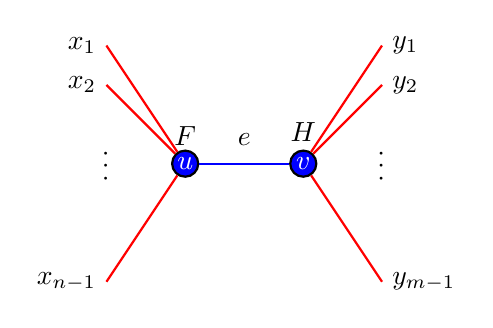
\begin{tikzpicture}[thick]
	%\ (f) at (0, 0) {$F$};
	\node (f) [circle, minimum size=0.1cm, draw=black,fill=blue] at (0,0) {} node [above=0.1cm] {$F$};
	\node (h) [circle, minimum size=0.1cm, draw=black,fill=blue] at (1.5,0) {} node at (1.5,0.4) {$H$};
	% \draw (1.5,0) coordinate (h) node [above] {$H$};
	\draw[-, color=blue] (f) -- (h);
	\node at (0.75,0.3) {$e$};
	\node [color=white, very thick] at (0, 0) {$u$};
	\node [color=white, very thick] at (1.5, 0) {$v$};

	\draw[-, color=red] (-1, 1.5) node [left,color=black] {$x_1$} -- (f);
	\draw[-, color=red] (-1, 1.0) node [left,color=black] {$x_2$} -- (f);
	\node [rotate=90] at (-1, 0) {$\cdots$};
	\draw[-, color=red] (-1, -1.5) node [left,color=black] {$x_{n-1}$} -- (f);
	
	\draw[-, color=red] (2.5, 1.5) node [right,color=black] {$y_1$} -- (h);
	\draw[-, color=red] (2.5, 1.0) node [right,color=black] {$y_2$} -- (h);
	\node [rotate=90] at (2.5, 0) {$\cdots$};
	\draw[-, color=red] (2.5, -1.5) node [right,color=black] {$y_{m-1}$} -- (h);

\end{tikzpicture}

\end{figure}
如图即为第一种基本张量网络,其中该网络有一条内部边$e$,顶点$u$,$v$对应的函数分别为$F(e,x_1,x_2,\\ \cdots,x_{n-1})$和$H(e,y_1,y_2,\cdots, y_{m-1})$。

$F$和$H$分别是n元和m元函数,则他俩合成的张量网络$S$是一个$n+m-2$元的函数$S(x_1,x_2,\cdots, \\x_{n-1}, y_1, y_2, \cdots, y_{m-1})$。该张量网络的所有边,即所有变元的定义域均为$D=\{0,1\}$。

我们要证明此开放张量网络的函数S是一个斐波那契门,即须证明S是对称函数,以及S的函数值满足递推关系$s_{i+2}=s_{i} + s_{i+1} $。

而证明$S$是对称函数的含义是,在输入为$i$个1和$n+m-2-i$个0时,$S$的函数值都相同(将其记做$s_i$)。

当张量网络$S$的输入为$i$个1和$n+m-2-i$个0,且其中的$j$个1来自于$F$的变元,另外$i-j$个1来自于$H$的变元时,将张量网络的函数值记为$s_{i,j}$。要证$S$是对称函数,即证$s_{i,0}=s_{i,1} = \cdots=s_{i,i} $

只需证明当$j = 1, 2, \cdots, i$时,都有$s_{i,j} = s_{i,j-1}$成立即可。

下面我们开始推导$s_{i,j}$的表达式。

由张量网络的定义知 $S=\sum_{e\in D}F(e,x_1,x_2,\cdots,x_{n-1})H(e,y_1,y_2,\cdots, y_{m-1})$

计算$s_{i,j}$:

\begin{equation*}
\begin{split}
s_{i,j} &= \sum_{e\in D}F(e,x_1,x_2,\cdots,x_{n-1})H(e,y_1,y_2,\cdots, y_{m-1}) \\
&= F(0,x_1,x_2,\cdots,x_{n-1})H(0,y_1,y_2,\cdots, y_{m-1})+F(1,x_1,x_2,\cdots,x_{n-1})H(1,y_1,y_2,\cdots, y_{m-1})\\
&=f_jh_{i-j} + f_{j+1}h_{i-j+1}
\end{split}
\end{equation*}

以$j-1$代$j$,得$s_{i,j-1}=f_{j-1}h_{i-j+1} + f_{j}h_{i-j+2}$
\begin{equation*}
\begin{split}
s_{i,j}-s_{i,j-1} &= (f_jh_{i-j} + f_{j+1}h_{i-j+1}) - (f_{j-1}h_{i-j+1} + f_{j}h_{i-j+2})\\ & = f_j(h_{i-j} - h_{i-j+2}) + h_{i-j+1}(f_{j+1} -f_{j-1})\\
&= f_j(-h_{i-j+1}) + h_{i-j+1}f_j\\
&= 0
\end{split}
\end{equation*}

故$S$是对称函数得证。且有$s_i = s_{i,0} = f_0h_i + f_1h_{i+1}$。

下证$S$满足递推关系$s_{i+2}=s_{i} + s_{i+1}$。
\begin{equation*}
\begin{split}
s_{i+2} &= f_0h_{i+2} + f_1h_{i+3}\\
&=f_0(h_{i}  + h_{i+1}) + f_1(h_{i+1} + h_{i+2})\\
&=(f_0h_i + f_1h_{i+1}) + (f_0h_{i+1} + f_1h_{i+2})\\
&=s_{i} + s_{i+1}
\end{split}
\end{equation*}

\begin{figure}[htbp]
	\centering
	\begin{tikzpicture}[thick]
		%\ (f) at (0, 0) {$F$};
		\node (a) [circle, minimum size=0.05cm, draw=black,fill=blue] at (0,0) {} node [above=0.1cm] {$A$};
		\node (b) [circle, minimum size=0.1cm, draw=black,fill=blue] at (0,-1) {} node at (1.5,0.4) {$B$};
		% \draw (1.5,0) coordinate (h) node [above] {$H$};
		\draw[-, color=blue] (f) -- (h);
		\node at (0.75,0.3) {$e$};
		%\node [color=white, very thick] at (0, 0) {$u$};
		%\node [color=white, very thick] at (1.5, 0) {$v$};

		\draw[-, color=red] (-1, 0) node [left,color=black] {$x_1$} -- (f);
		\draw[-, color=red] (-1, 1.0) node [left,color=black] {$x_2$} -- (f);
		\node [rotate=90] at (-1, 0) {$\cdots$};
		\draw[-, color=red] (-1, -1.5) node [left,color=black] {$x_{n-1}$} -- (f);
		
		\draw[-, color=red] (2.5, 1.5) node [right,color=black] {$y_1$} -- (h);
		\draw[-, color=red] (2.5, 1.0) node [right,color=black] {$y_2$} -- (h);
		\node [rotate=90] at (2.5, 0) {$\cdots$};
		\draw[-, color=red] (2.5, -1.5) node [right,color=black] {$y_{m-1}$} -- (h);

	\end{tikzpicture}

\end{figure}
\begin{figure}[htbp]
	\centering
	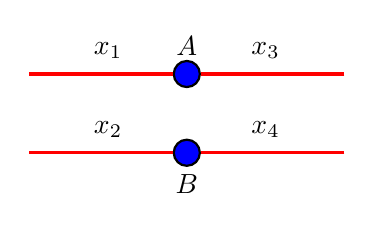
\begin{tikzpicture}[thick]
		\node (a) [circle, minimum size=0.05cm, draw=black,fill=blue] at (0,0) {} node [above=0.1cm] {$A$};
		\draw[-, color=red, very thick] (-2,0)  --(a);
		\node at (-1, 0.3) {$x_1$};
		\draw[-, color=red, very thick] (2,0)  --(a);
		\node at (1,0.3) {$x_3$};

		\node (b) [circle, minimum size=0.1cm, draw=black,fill=blue] at (0,-1) {} node at (0,-1.4) {$B$};
		\draw[-, color=red, very thick] (-2,-1)  --(b);
		\node at (-1, -0.7) {$x_2$};
		\draw[-, color=red, very thick] (2,-1)  --(b);
		\node at (1,-0.7) {$x_4$};

	\end{tikzpicture}

\end{figure}

\begin{figure}[htbp]
	\centering
	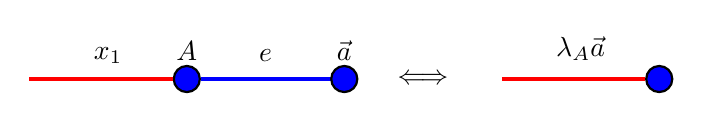
\begin{tikzpicture}[thick]
		\node (A) [circle, minimum size=0.05cm, draw=black,fill=blue] at (0,0) {} node [above=0.1cm] {$A$};
		\draw[-, color=red, very thick] (-2,0)  --(A);
		\node at (-1, 0.3) {$x_1$};
		\draw[-, color=blue, very thick] (2,0)  --(A);
		\node at (1,0.3) {$e$};
		\node (a) [circle, minimum size=0.05cm, draw=black,fill=blue] at (2,0) {} node [above=0.1cm] at (2,0) {$\vec a$};
		
		\node at (3,0) {$\iff$};

		\node (a') [circle, minimum size=0.05cm, draw=black,fill=blue] at (6,0) {} node [above=0.1cm] at (5,0) {$\lambda_A\vec a$};	
		\draw[-, color=red, very thick] (4,0)  --(a');
		
	\end{tikzpicture}

\end{figure}
\begin{figure}[htbp]
	\centering
	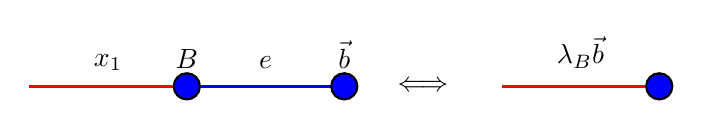
\begin{tikzpicture}[thick]
		\node (B) [circle, minimum size=0.05cm, draw=black,fill=blue] at (0,0) {} node [above=0.1cm] {$B$};
		\draw[-, color=red, very thick] (-2,0)  --(B);
		\node at (-1, 0.3) {$x_1$};
		\draw[-, color=blue, very thick] (2,0)  --(B);
		\node at (1,0.3) {$e$};
		\node (b) [circle, minimum size=0.05cm, draw=black,fill=blue] at (2,0) {} node [above=0.1cm] at (2,0) {$\vec b$};
		
		\node at (3,0) {$\iff$};

		\node (b') [circle, minimum size=0.05cm, draw=black,fill=blue] at (6,0) {} node [above=0.1cm] at (5,0) {$\lambda_B\vec b$};	
		\draw[-, color=red, very thick] (4,0)  --(b');
		
	\end{tikzpicture}

\end{figure}
\begin{figure}[htbp]
	\centering
	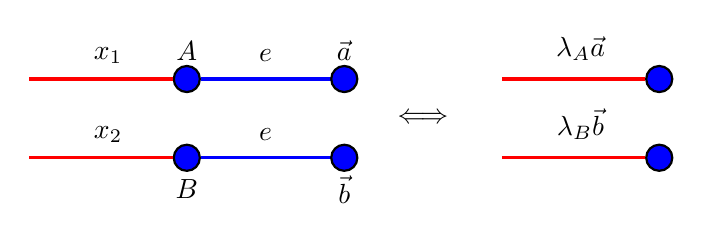
\begin{tikzpicture}[thick]
		\node (A) [circle, minimum size=0.05cm, draw=black,fill=blue] at (0,0) {} node [above=0.1cm] {$A$};
		\draw[-, color=red, very thick] (-2,0)  --(A);
		\node at (-1, 0.3) {$x_1$};
		\draw[-, color=blue, very thick] (2,0)  --(A);
		\node at (1,0.3) {$e$};
		\node (a) [circle, minimum size=0.05cm, draw=black,fill=blue] at (2,0) {} node [above=0.1cm] at (2,0) {$\vec a$};
		\node (a') [circle, minimum size=0.05cm, draw=black,fill=blue] at (6,0) {} node [above=0.1cm] at (5,0) {$\lambda_A\vec a$};	
		\draw[-, color=red, very thick] (4,0)  --(a');
		
		\node at (3,-0.5) {$\iff$};

		\node (B) [circle, minimum size=0.1cm, draw=black,fill=blue] at (0,-1) {} node at (0,-1.4) {$B$};
		\draw[-, color=red, very thick] (-2,-1)  --(B);
		\node at (-1, -0.7) {$x_2$};
		\draw[-, color=blue, very thick] (2,-1)  --(B);
		\node at (1,-0.7) {$e$};
		\node (b) [circle, minimum size=0.05cm, draw=black,fill=blue] at (2,-1) {} node [below=0.1cm] at (2,-1) {$\vec b$};
		\node (b') [circle, minimum size=0.05cm, draw=black,fill=blue] at (6,-1) {} node [above=0.1cm] at (5,-1) {$\lambda_B\vec b$};	
		\draw[-, color=red, very thick] (4,-1)  --(b');

	\end{tikzpicture}

\end{figure}

\end{document}
